% % % % % % % % % % % % % % % % % % % % % % % % % % % % % % % % 
% BSc Physics Dissertation
% % % % % % % % % % % % % % % % % % % % % % % % % % % % % % % %
\documentclass[twoside, fontsize=12pt,
     bibliography=totoc, % Include bibliography in contents
     listof=totoc, % Include lists of figures and tables in contents
     index=totoc, % Include index in contents
     onehalfspacing %  or doublespacing
    %,openright
]{_MScDiss2017_cls}

%\usepackage{txfonts,epsfig}
\usepackage[labelfont=footnotesize,textfont=footnotesize]{caption}   
\usepackage{_twoopt}
\usepackage{url}
\usepackage{breakurl}
\usepackage[]{_MScDiss_sty}
%\usepackage{chngcntr}
%\counterwithout{footnote}{chapter}

%% these macros turn citations into ADS clickers in dvi, pdf, html output
%% (EDP Sciences improved them in December 2012 to work also with pdflatex)
\bibpunct{(}{)}{;}{a}{}{,}    %% natbib cite format used by A&A and ApJ
\makeatletter
 \newcommandtwoopt{\citeads}[3][][]{\href{http://adsabs.harvard.edu/abs/#3}%
   {\def\hyper@linkstart##1##2{}%
    \let\hyper@linkend\@empty\citealp[#1][#2]{#3}}}    %% Rutten, 2000
 \newcommandtwoopt{\citepads}[3][][]{\href{http://adsabs.harvard.edu/abs/#3}%
   {\def\hyper@linkstart##1##2{}%
    \let\hyper@linkend\@empty\citep[#1][#2]{#3}}}      %% (Rutten 2000)
 \newcommandtwoopt{\citetads}[3][][]{\href{http://adsabs.harvard.edu/abs/#3}%
   {\def\hyper@linkstart##1##2{}%
    \let\hyper@linkend\@empty\citet[#1][#2]{#3}}}      %% Rutten (2000)
 \newcommandtwoopt{\citeyearads}[3][][]%
   {\href{http://adsabs.harvard.edu/abs/#3}%
   {\def\hyper@linkstart##1##2{}%
    \let\hyper@linkend\@empty\citeyear[#1][#2]{#3}}}   %% 2000
\makeatother

\declaration{I hereby certify that this Dissertation, which is approximately N thousand words in length, has been written by me at the School of Physics and Astronomu, Queen Mary University of London, that all material in this dissertation which is not my own work has been properly acknowledged, and  that it has not been submitted in any previous application for a higher degree.\\ \\
The sections which contain the report on the independent research work component of the project are Sections X.X, Y.Y-Z.Z, and Q.Q.} 

%--Put your information between here----%
\title{your Dissertation Title}
\author{your Name (student number in brackets) }
\supervisor{your supervisor's Name}
%\date{\today}
\date{31 August 2017}
%\acknowledgements{} 
\acknowledgements{I  thank whoever I want here - or I can instead comment it out.}
\newpage% to ensure page 1 starts on front of a page rather than back
%---and here------%

\begin{document}
\pagenumbering{roman}
\setcounter{tocdepth}{5}

\maketitle
\abstract{The origin of the Universe is modeled.}
\tableofcontents % generates Table of Contents
\listoffigures % generates List of figures
\listoftables % generates List of Tables

\newpage% to flush out last roman numeral
\cleardoublepage
\pagenumbering{arabic}% Set arabic page numbers now that dissertation proper is starting.

% rather than having a very long file you can Input files for each chapter/section here using 
% \input{relative-path-to-file} or just put the files in the same directory as this file.

%Chapter
\chapter{The Dissertation Template}
\label{sec:template}
Your MSc dissertation should be produced in LaTeX and have filename \newline Surname\_MScDiss2017.pdf (where surname should be replaced by your Surname - this example file uses Surname instead of your Surname).

This document, and its associated files, provides a template and for your submission and includes some examples of features of \LaTeX. 
This template handles the required information at the start of a Dissertation (see \ref{sec:preamble}) and you should use the  version in folder 2017\_MScDissTemplate\_NoContent (see below) as the starting point of your assessed report. 

This document is the output from running TeXworks on file \newline  Surname\_MScDiss2017.tex \newline in folder \newline 2017\_MScDissTemplate\_ExampleContent

The files in 2017\_MScDissTemplate\_ExampleContent show an example of how to introduce figures, how to refer to other parts (e.g. Figures, Tables, Sections etc etc) of the dissertation (clicking on the blue name of a cross reference in the pdf will jump to the label in the pdf, and on an url will go to that url, and on a reference will go to the NASA Astrophysics Data System (ADS) entry for that peper see 
Section~\ref{sec:features}), but - very importantly - it shows how to produce properly formatted references in a bibliography using BibTeX. 

The files in 2017\_MScDissTemplate\_NoContent provide an empty template for your Dissertation submission.  Note that even this empty template reads in and uses the 6 files prefixed with an underscore \_ namely:
\begin{itemize} 
\item \_abbrvnat\_jpe.bst
\item \_jnls.cls
\item \_MScDiss2017\_cls.cls
\item \_MScDiss2017\_Preamables.cls
\item \_MScAstroDiss\_sty.sty
\item \_twoopt.sty
\end{itemize}
so be careful never to delete, or change the names of, any of these 6 files or your typesetting will always fail. 

\section{Citation features provided by template} 
\label{sec:features}
A very useful citation-related feature of this template is that clicking on the citation will take you to the ADS web page for the citation, {\em if the citation is from ADS. This does not work for non ADS citations} -  see Chapter \ref{chap:bibtex}. This gives the pdf version of your report useful connectivity to the references - rather like in an online journal. 

The slight downside is that you have to refer to the paper in the text by the rather unmemorable name assigned by ADS. If you change the unmemorable name the link to ADS will no longer work (because the unmemorable name is used to make the link to ADS). This seems a small price to pay for not having to type in (and probably also correct) all the information yourself!

\section{Template with preambles etc}
\label{sec:preamble}
At the start of this version here there are pages with Title page, Declaration, Acknowledgments (optional), Abstract, Contents and Lists of Figures and Tables. When working on your draft you may not want to have to see these every time. To temporarily suppress (don't forget to undo this for the submited version) the Declaration \& Acknowledgments  open MScDiss2017\_cls.cls in a text editor, and change
\begin{verbatim} \input{MScDiss2017_Preambles.cls} % uncomment for submission \end{verbatim}
 to 
 \begin{verbatim}% \input{MScDiss2017_Preambles.cls} % uncomment for submission \end{verbatim}
 
To temporarily suppress the Title page, Abstract, Table of Contents, and Lists of Figures and Tables put a \% in front of the following 5 commands in this .tex file - this has the effect of commenting them out. 
\begin{verbatim}
\maketitle

\abstract{The origin of the Universe is modeled.}
\tableofcontents % generates Table of Contents
\listoffigures % generates List of figures 
\listoftables % generates List of Tables
\end{verbatim}
 
 {\normalfont\itshape Remember to uncommented all these for your actual submission, and to add the number of words and the sections with independent research to the Declaration}  All these are needed for the submitted Dissertation

If you don't want an Acknowledgments section in the submitted version then just leave the space between the \{\} empty  in 
\begin{verbatim}\acknowledgements{}\end{verbatim}

\subsection{Pagination}
\label{subsec:sides}
Note that the odd numbered pages should have the wide vertical margin (for binding) on the left hand side of the page and page number in bottom right. After you have included the preamble material, and Table of Contents and the Lists of Figures and Tables will have expanded and they may take up an odd number of pages in which case page 1 may no longer have the wide vertical margin (for binding) on the left hand side of the page and page number on the right. If this happens to you contact Prof Emerson for a solution before you submit.
%end Chapter

%Chapter
\chapter{\LaTeX }
\section{Installing \LaTeX}
I recommend using TeXworks to edit and run LaTeX files. You should install TeXworks on your personal laptop/pc for working at home. It should already be installed on the machines in the MSc room (GO Jones 230).
 
\begin{itemize}
\item for Windows or Linux machines install TeXLive which includes TeXworks - see \url{https://www.tug.org/texlive/} 
\item for Mac OSX machines install MacTeX which includes TeXworks - see \url{http://tug.org/mactex/}. MacTeX also includes TeXShop (for Macs only), on which TeXworks is based. Stick to using TeXworks so we are all using the same package whether we work in Windows, Linux or Mac.
\item if you are already familiar with some other version of LaTeX you may stick with it.
\end{itemize}

After installing TeXworks open Preferences and chose Editor (see Fig \ref{fig:texworks-prefs}) and under 'Syntax coloring' chose LaTeX - this should help in seeing what is a LaTeX command and what is not and where the \{s and their corresponding \}s are. When you have installed spell checking (see \ref{sec:spell}) chose English as the language here.
You can set the default font and font size but these will be overriden by the values set by the template.

\begin{figure}[hbtp]
  \begin{center}
  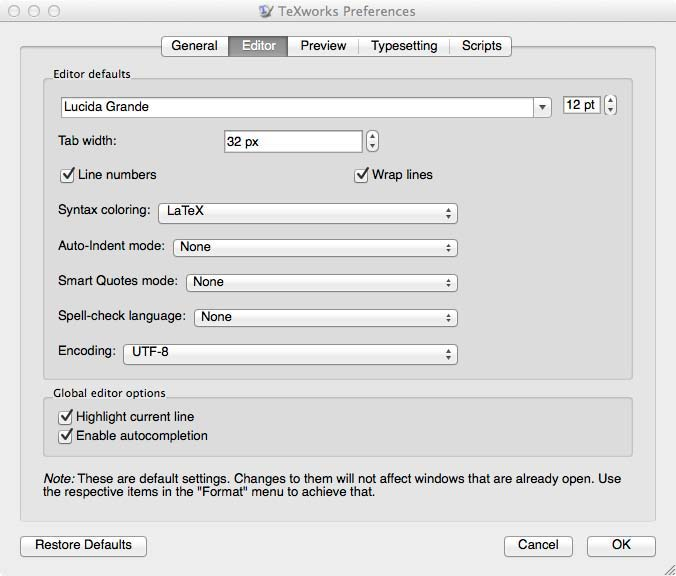
\includegraphics[width=80mm]{fig-texworks-preferences-editor.jpg}  %% file name without extension
  \caption{Screen shot (on a Mac) of TeXworks preferences for Editor} 
  \label{fig:texworks-prefs}
  \end{center}
\end{figure}

\subsection{Spell checkers for LaTeX}
\label{sec:spell}
TeXworks does not currently include any bundled spelling dictionaries, so if you want spell-checking to be enabled in the editor, as is likely, you need to install dictionaries separately. An easy source of English (and other) dictionaries is the OpenOffice.org project at \url{http://extensions.services.openoffice.org}. Download {\normalfont\itshape English dictionaries for Apache Open Office}. Rename the downloaded dict-en.oxt file to dict-eng.zip; extract the spelling dictionary *en\_GN*.dic and en\_GB.aff files as TeXworks can only use the *.dic and *.aff files. Consult the instructions at \url{http://code.google.com/p/texworks/wiki/SpellingDictionaries} for where to put the *.dic and *.aff files.

MicroSpell \url{http://www.microspell.com/fixmytypos.html}  is an online Spell Checker which accepts LaTeX.
Or one could convert the pdf to text and spell check the text in Microsoft Word. Some other LaTeX editors have spell checkers (for a list see 
\url{http://tex.stackexchange.com/questions/339/latex-editors-ides}). 

\subsection{Word counters for LaTeX}\label{sec:count}
TeXcount \url{http://app.uio.no/ifi/texcount/} offers a web based LaTeX word count both using a downloadable script and as a web service.

An alternative approach is to count the words in the PDF file output from LaTeX.
WordCounter \url{http://www.docwordcounter.com} is a free online word counter that counts and classifies the words in your PDF, Word, and standard text files.

\url{http://freenuts.com/free-online-word-count-tools/} lists other word counting tools, or you can google 'pdf word count free' to find ones that all work with pdfs. 

You can also do it yourself by converting a copy of the pdf to plain text, reading it into Microsoft Word and then using Word to do the counting.
%end Chapter

%chapter
\chapter{BiBTeX}
\label{chap:bibtex}
\section{Gathering citations in BiBTeX format}
\label{sec:gather}
The bibliography for your  dissertation should use BibTeX which uses .bib files. You can read about these by googling BibTeX but you shouldn't need to do this  \underline{assuming that }all your references can be found on the NASA ADS site, which will usually be the case. If any  citations are not there (only a few I hope) then you should be able to download a BibTeX file from the Journal instead (e.g. see BiBTeX files bib-aanda.bib,  bib-apj.bib, bib-astronj.bib, bib-mnras.bib in this package). However these will behave differently from an  BibTeX file from ADS because it has some fields which are different e.g. instead of an  {\normalfont\bfseries adsurl} field (see ads.bib) they have a {\normalfont\bfseries url} field (see bib-apj.bib)  etc etc.

For a reference you want to refer to:
\begin{itemize}
\item Find it on the NASA ADS  \url{http://ukads.nottingham.ac.uk/abstract_service.html} 
e.g. Whittet, D.  searched 1993 to 1993 produces 15 abstracts. Suppose you want no 14 \citepads{1993dca..book....9W} which is an article in a book.
Actually it is not a very well formed reference but was picked so Fig \ref{fig_bibads} would be quite short - click the blue number after Fig above (in the line above) and see what happens.
%===========================================================================
\begin{figure}[hbtp]
  \centering
  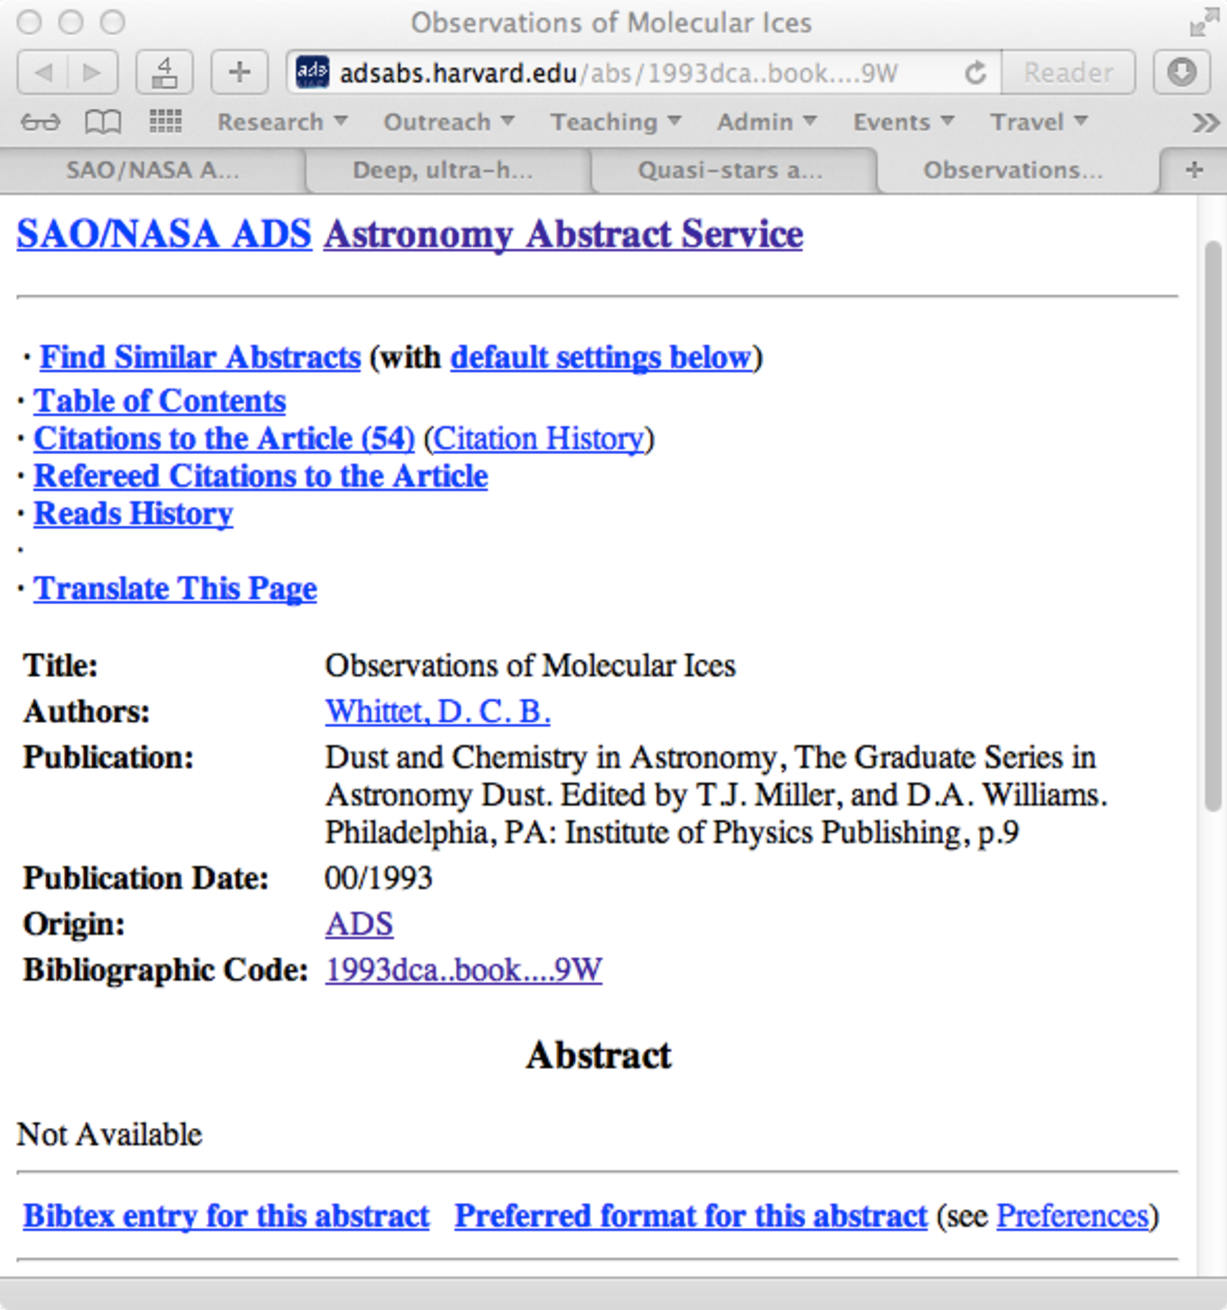
\includegraphics[width=70mm]{fig-bib}  %%  %% file name with or without extension
  \caption[Get BibTeX format reference from ADS.]% the caption in [] appears in List of Figures is an abbreviated caption for the List of Figures as the actual caption is so long.
  {In ADS click on bottom left link 'Bibtex entry for this abstract' to get the BibTeX format reference.}% the caption in {} appears in the text and can be longer than the abbreviated one for the list
  \label{fig_bibads}
\end{figure}
%===========================================================================
\item In ADS after the Abstract etc there is a Printing Options section, More Article Retrieval Options, HELP for Article Retrieval, and then "Bibtex entry for this abstract" see Fig \ref{fig_bibads}. 
\item Click on \lq Bibtex entry for this abstract\rq. Cut and Paste the BiBteX format reference into a plain text file with name Surname.bib (whre Surname is your surname) along with the other references you have got in the same way.  One could have a string of .bib files with any unique names you like as long as they end in .bib, or just one .bib file. here I have prefaced all .bib file names except surname.bib with bib- so they appear in together in an alphabetically sorted directory list.
\end{itemize}

The structure you found above is for a journal article - there are analogous (but different) structures for Books, Conferences etc etc. 
Various formats are provided by BibTeX including the following  
\begin{itemize}{}
\item Journal articles e.g. An important Cosmology paper   \citetads{1965ApJ...142..419P}  which got the Nobel prize.
\item Conference proceedings e.g. Amongst the many papers in  \citetads{1999ASPC..168.....T} (conference proceedings) there is one of great interest to this study  \citetads{1999ASPC..168..461W}(one paper in the proceedings). 
\item Books e.g.  In  \citetads{1993dca..book.....M} (a book) there are many interesting papers including  \citetads{1993dca..book....9W} (one paper in the book).
\item PhD theses e.g. \citetads{2012PhDT.........1B},  
\item Preprints e.g. \citetads{2012arXiv1211.2860S}. N.B.  Only recent preprints should be used, and then only if the paper itself  has not yet appeared in the Journal by the time of submission. (In most cases ancient reprints are not suitable as references as they were (if still only available as a preprint) presumably never published.)
\item Technical Reports e.g. \citetads{1993cuny.reptS....H}
\end{itemize}

The 2 main example .bib files  for this template's bibliography were made by downloading citations from ADS as described above into bib-stateqm.bib and bib-various.bib, e.g.  \citetads{1994IAUS..154..309R}. 

In this template there is also one reference each whose .bib entry was got from the websites of:  MNRAS (see bib-mnras.bib for \citetads{MNR:MNR20111}); ApJ (see bib-apj.bib for \citetads{0004-637X-672-1-198}; AstrJ (see bib-astrj.bib for \citetads{1538-3881-143-3-70}); and A\&A(see bib-aanda.bib for \citetads{refId0}). Note that for these, which don't come from ADS, the  link doesn't work (as non-ADS .bib entries  do not contain the right name for ADS to find them). However they do produce the url for the link at end of the printed reference at the end.

Open all the .bib files with a text editor and look at their structure, and at the corresponding References that appear in the pdf. You should see the logic of them, and how you could make a BiBTeX reference yourself - but the beauty is that by using the ADS you don't actually have to!

A bibtex entry for a book (if you have to make one) might look something like this.
\begin{verbatim}
@Book{Conway2000,
author = {Damian Conway},
title = {Object {O}riented {P}erl: {A} comprehensive guide to programming},
publisher = {Manning Publications Co.},
year = {2000},
address = {Connecticut, USA}
}
\end{verbatim}
and would come out \cite{Conway2000}

\subsection{Aids to Citation Gathering}
\label{subsec:aids}
You may wish to make your  library of .bib files easier to mange using one of various free citation library management tools that work with BiBTeX. These include Zotero (\url{http://www.zotero.org}) which is an add-on to Firefox and JabRef (\url{http://jabref.sourceforge.net}) which is written in Java and so will run on any platform (windows, linux, mac).

\section{Making references in LaTeX}\label{sec:referencing}
To use your  bibliography (7 .bib files in this example - you may have a differnt bumber but you need at least one)

\begin{itemize}
\item Put \textbackslash  bibliography\{Surname.bib, bib-stateqm,bib-various,bib-aanda,bib-apj,bib-astronj,bib-mnras\} near the end (see LaTeX source for this document) replacing these .bib files with your list of .bib files. (You don't need the .bib suffixes in \textbackslash  bibliography\{\}).
\item to cite a paper in the \underline{text} use (e.g.) \textbackslash citetads\{2010MNRAS.408..342B\}  where the value in curly brackets is the ADS reference name. e.g.  \citetads{2010MNRAS.408..342B}.
\item to cite cite a paper in \underline{parentheses} use (e.g.) \textbackslash citepads\{2010MNRAS.408..342B\}  where the value in curly brackets is the ADS reference name e.g. \citepads{2010MNRAS.408..342B}.
\item to (unusually) cite a paper  \underline{by year} without the name being automatic use (e.g.) Biggs(\textbackslash citeyearads\{2010MNRAS.408..342B\} ) where the value in curly brackets is the ADS reference name e.g. Biggs(\citeyearads{2010MNRAS.408..342B}) - but this produces no link.
\end{itemize}

\subsection{What about \textbackslash cite\{\}?} 
\label{subsec;cite}
The standard citation command \textbackslash cite\{\} will also work but a) is not recommended and b) does not provide the link to ADS but instead jumps to that reference at the end of the document e.g. \cite{1993dca..book....9W}. 

If something were only to appear in printed form \textbackslash cite\{\} is all you would need, but if it will also be pdf (as in most cases) then use use of  \textbackslash citetads\{\}  or \textbackslash citepads\{\}  gives the active references e.g. \citetads{1993dca..book....9W} or \citepads{1993dca..book....9W}.

For referring to things such as a web page (in this case a link to the url of some course notes) you can use for example  \cite{QMULExtrasolarPlanetlecturenotes} which, as not on NASA ADS, will not link directly to the web page. So one uses \textbackslash cite to instead jump to the reference in the bibliography at the end of the dissertation from where you can go to the url - take a look at the final entry in bib-various.bib to see how this was constructed.

\section{Running LaTex with BibTex}
\label{sec:running}
Assume you have a document, called \lq Surname\_MScDiss2017.tex\rq , along with bibtex database(s), "surname, bib-x....x.bib" etc , which have been made as described in \ref{sec:gather} above. To completely process the document execute the following commands, in sequence:

\begin{itemize}{}
\item {\normalfont\bfseries pdflatex} Surname\_MScDiss2017  - generates various auxiliary files, 
\newline \lq \_Surname\_MScDiss2017.aux. .dep, .log, .out, .synctex.gz, .toc\rq , containing information about citations (and other types of references), the bibliography style used, and the name of the bibtex database. 
\item {\normalfont\bfseries bibtex} Surname\_MScDiss2017  - uses the information in the auxiliary files, along with the data contained in the .bib files, to create a file\\ \lq \_Surname\_MScDiss2017.bbl\rq\, and .blg containing a \lq thebibliography\rq\, environment with \lq bibitem\rq\, entries formatted according to the bibliography style specified.
\item {\normalfont\bfseries pdflatex}  Surname\_MScDiss2017 - runs  the paper again through LaTeX, now updates the auxiliary files.
\item {\normalfont\bfseries pdflatex}  Surname\_MScDiss2017 - produces the final  output automatically giving the references in the right form in the text and the right order in the bibliography. 
\end{itemize}

i.e. run pdflatex once, BiBTeX once, and then pdflatex twice more.

Note the following.
\begin{itemize}{}\item It does not matter what order the papers are in the .bib files (so no need to spend time making them alphabetical).
\item Multiple papers by the same author in the same year are automatically handled  by adding a letter to the year. e.g.\citetads{1936ApJ....84..158H}, \citetads{1936ApJ....84..270H} or \citepads{1936ApJ....84..158H,1936ApJ....84..270H}. 
\item A reference that appears twice is warned as a repeating entry but handled OK. 
\item Any references in the .bib files that are not referenced do not appear.
\item If a reference is cited that is not in the .bib files an error will be reported. 
\item Some entries, even amongst those downloaded from ADS,  generate warning messages if information that should be present  is not, or if there is unrecognised information  e.g.
\begin{verbatim}
Repeated entry---line 134 of file various.bib
 : @article{1965ApJ...142..419P
 :                             ,
I'm skipping whatever remains of this entry
Warning--empty institution in 1993cuny.reptS....H
Warning--empty publisher in 1993dca..book.....M
Warning--can't use both author and editor fields in 1993dca..book....9W
Warning--empty publisher in 1993dca..book....9W
\end{verbatim}
BibTeX will not usually fail because of this but you should reassure yourself that there are obvious bad effects in the Bibliography at the end of your Dissertation. To be useful a reference must obviously be findable from the information in the reference! You can correct any such problems by hand if necessary by editing of the problematic .bib entries.
\end{itemize}
%end Chapter

%Chapter
\chapter{Nonsense Chapter }
\label{ch:eqm}
This is some dummy/nonense content showing cross references, figure, table, numbered formulae and references using BiBTeX

After the recession of distant galaxies beyond our Local Group of galaxies  was discovered  \citepads{1929PNAS...15..168H} some  resisted the idea of the Hot Big Bang on philosophical grounds even after the discovery of Cosmic Microwave Background radiation (CMB) by \citetads{1965ApJ...142..419P}. 

This has got absolutely nothing to do with Section \ref{sec:gather} or with Fig \ref{fig:waterfalls} but click on the blue text\footnote{Note that clicking on the blue name of any labelled link in the pdf will jump to the label in the pdf (e.g. to the section, figure, table) or (if the reference's .bib entry was downloaded from ADS) to the reference on ADS as long as you are connected to the internet.}
and note the effects which are very useful in a pdf (though of no use in plain print). 

This paragraph is true - not nonsense! Figures and tables are called floats: they can float around in the document and LaTeX will try to judge the best place to put them. Don't waste time tring to force them to be in a particualr place!

%% {fig:waterfalls}
%===========================================================================
\begin{figure}[hbtp]
\begin{center}
  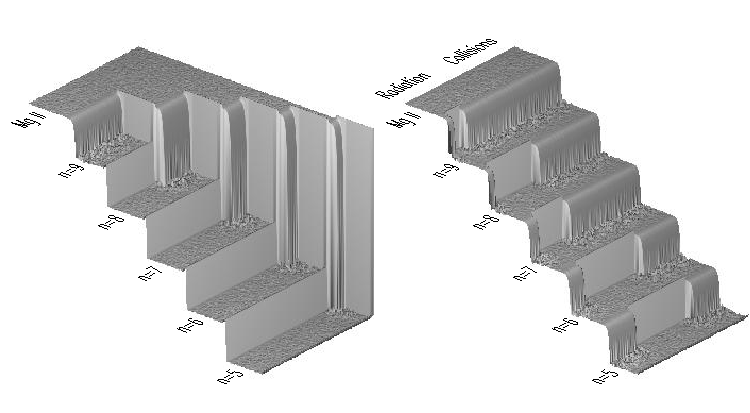
\includegraphics[width=155mm]{fig_waterfalls}  %% file name with or without extension
  \caption[ Collisional-radiative recombination along Mg\,I Rydberg states ]% the caption in [] appears in List of Figures is an abbreviated caption for the List of Figures as the actual caption is so long.
 { Collisional-radiative recombination along Mg\,I Rydberg states
    visualized for kayakers.  The largest recombination flow from the
    magnesium population reservoir in the Mg\,II ground state is into
    the highest level ({\em left\/}, showing the relative rates from
    the continuum into different Rydberg levels).  The downward
    population flow from the highest level is largest along the
    cascade with $\Delta n \!=\!1$ steps (not shown).  
    %% \! for less space around =
    The recombination flow is initially dominated by collisional
    transitions ({\em right\/}, showing the division between radiative
    and collisional transitions for recombination into $n\!=\!9$ and
    along the $\Delta n \!=\!1$ ladder).  The flow is driven by photon
    losses in strong lines lower in the Mg\,I term structure and is
    balanced by radiative ionization to Mg\,II in ultraviolet edges.
    From \citetads{1994IAUS..154..309R}. 
    } % the caption in {} appears in the text and can be longer than the abbreviated one for the list
\label{fig:waterfalls}
\end{center}
\end{figure}   
%===========================================================================

\section{The Development of the Field}
\label{sec_devel}
This section describes the development of the  field. The field was introduced in Section~\ref{ch:eqm}.

This is a new paragraph. {\normalfont\bfseries Note} that the first paragraph of a 
section is not indented, but later paragraphs are indented. 

\section{Data}
\label{sec:data}
This data analysed is based on the  HST images of OMC1 in Figure~\ref{orion_pic} and the dat in Table~\ref{tab:meth}. 
%===========================================================================
\begin{figure}[hbtp]
\begin{center}
 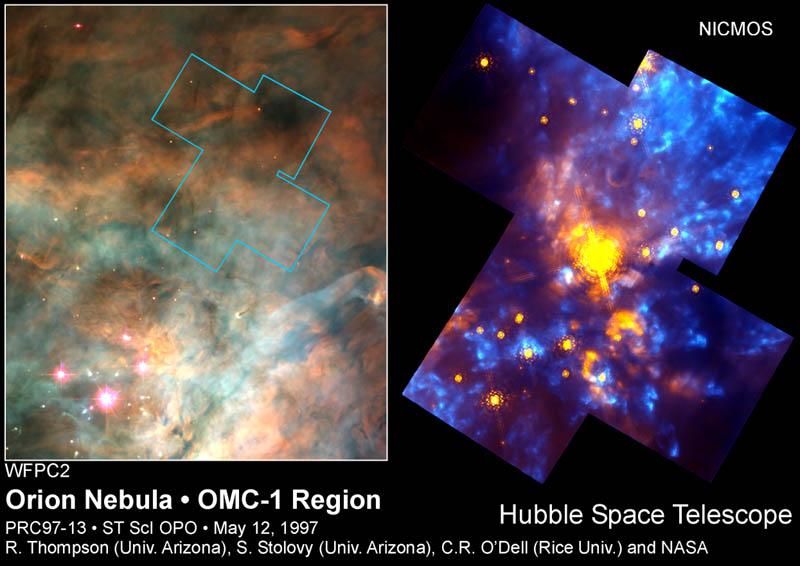
\includegraphics[height=70mm]{fig-omc1nic}
 \caption {Orion Molecular Cloud 1 - image from HST's NICMOS}
 \label{orion_pic}
\end{center}
\end{figure}
%===========================================================================
\section{The Method}
\label{sec_method}
This section describes the method. The field was introduced in Section~\ref{sec_devel} 
and the results are based on Equarion~\ref{eqn10}. 

The methods used the equation $p = \alpha + 7$ which is then used 
to calculate the factor 
\begin{equation}
 f = \frac{p+1}{ \sqrt{ p + \log( p^2 + 3 ) } }  . 
 \label{eqn10}
\end{equation}
This is then used to calculate 
\begin{equation}
 \beta = \frac{1}{ \sqrt{ f + 4 } } .
 \label{eqn5}
\end{equation}
Note that Equation~\ref{eqn10} has a label, as does Equation~\ref{eqn5}. 

This equation is surrounded by double dollars in the .tex file, 
which means that it does not have a number in the final document. 
$$   
 \gamma = \Delta p \cos{ p }
$$
Double dollars puts the equation on its own line, while single 
dollars puts $\gamma = \Delta p \cos{ p }$ in the text. 

The result of the methods are listed in Table~\ref{tab:meth}. 
%===========================================================================
\begin{table}
 \begin{center}
 \begin{tabular}{|c|c|c|} \hline
 Method & Description & Usefulness \\ \hline
 1  &  First method  & Failed \\ \hline
 2  &  Second method & Failed \\ \hline
 3  &  Third method  & Failed \\ \hline
 4  &  Fourth method & Failed \\ \hline
 5  &  Fifth method  & Worked \\ \hline
 \end{tabular}
 \caption{This is a dummy table }
 \label{tab:meth}
 \end{center}
\end{table}
%===========================================================================

\subsection{Lists}
\label{subsec_list}
This subsection contains a numbered list
\begin{enumerate} 
 \item Fish
 \item Meat
 \item Vegetables
\end{enumerate}
Or one could use letters instead of numbers.
%end Chapter

%%%%%%%%%%%%%%%%%%%%%%%%%%%%%%%%%%%%%%%%%%%%%%%%%%%%%%%%%%%%%%%%%%%%
%%BIBLIOGRAPHY SECTION
\begin{singlespace}% Start single space for bibliography
\bibliographystyle{_abbrvnat_jpe}    
\bibliography{Surname,bib-aanda,bib-apj,bib-astronj,bib-mnras,bib-stateqm,bib-various} %makes BIBLIOGRAPHY from the listed bib files  
\end{singlespace}

\end{document}
